\documentclass[11pt,a4paper]{article}
\usepackage[T1]{fontenc}
\usepackage[utf8]{inputenc}
\usepackage{lmodern,amsmath,amssymb,booktabs,array,graphicx}
\usepackage[margin=25mm]{geometry}
\usepackage{microtype,tikz,pgfplots}
\usetikzlibrary{arrows.meta,positioning}
\pgfplotsset{compat=1.18}
\usepackage[colorlinks=true,linkcolor=blue!45!black,citecolor=blue!45!black,urlcolor=blue!45!black]{hyperref}
\usepackage{caption}
\captionsetup{font=small,labelfont=bf}
\setlength{\parskip}{4pt}
\setlength{\parindent}{1em}
\setlength{\emergencystretch}{2em}
\newcommand{\pos}[1]{[#1]_{+}}
\newcommand{\R}{\mathbb{R}}
\newcommand{\ind}{\mathbf{1}}
\title{Trust-Gated Digital Twin Dispatch for Distribution Networks under Degraded Measurements}
\author{Chandrasen Pandey\\[4pt]
\small School of Computer Science, University of Petroleum and Energy Studies,\\
\small P.O. Bidholi, via Prem Nagar, Dehradun 248007, Uttarakhand, India\\
\small Corresponding author: \href{mailto:chandrasen.pandey@ddn.upes.ac.in}{chandrasen.pandey@ddn.upes.ac.in}}
\date{}
\begin{document}
\maketitle
\begin{abstract}
Digital twin dispatch depends on the quality of the measurements used to predict network conditions. This paper develops a causal trust gate for hourly battery dispatch in distribution networks. Measurement freshness, completeness, completed forecast residuals and independent meter agreement determine full dispatch, half-power dispatch or a hold. Each issued command receives an alternating-current (AC) power-flow check, while realised network conditions are assessed separately. Experiments use an IEEE 33-bus feeder and a 97-bus SimBench network, six chronological test blocks, six operating conditions and three random seeds. The design contains 62,208 controller evaluations. Across the equally weighted conditions, the trust gate reduces plant constraint violations from 0.797\% to 0.386\% on the 33-bus feeder and from 0.077\% to zero observed violations on the SimBench network. Mean energy-adjusted cost increases by 12.17 and 96.70 euros per 72-hour block, respectively. Authorisation coverage is 88.99\%, while non-zero dispatch is more frequent than with the ungated controller. At matched coverage, a simpler agreement score provides lower selective constraint risk. The results support a measured trade-off between cautious dispatch, operating cost and network feasibility. They also show that a composite trust score and an AC model check do not provide a general safety guarantee.
\end{abstract}
\noindent\textbf{Keywords:} Digital twin; Distribution network; Battery dispatch; Measurement quality; Prediction uncertainty; Power flow

\section{Introduction}\label{sec:intro}
Distribution networks with local generation and battery storage require control decisions that remain useful when measurements are incomplete, delayed or inconsistent. A digital twin can combine a network model with forecasts and operating records to support these decisions. The value of this combination depends on the information available when a command is issued. A forecast can appear accurate in an offline assessment while providing poor support for a particular dispatch decision. The resulting problem concerns both measurement quality and the physical consequences of control.

Digital twins for energy systems address modelling, data exchange and computational coordination \cite{ardebili}. Recent work in this journal has demonstrated a hardware-in-the-loop twin for analysing anomalies in a photovoltaic, hydrogen and storage system \cite{hueros}. Such developments establish the relevance of a digital representation connected to operating data. A separate requirement arises when the representation is used to authorise an action: evidence about the current data must be available before the action, and the resulting network state must be assessed independently.

\subsection{Operational problem and research question}
Measurement faults can affect dispatch through several paths. Missing observations remove recent information, delayed observations describe an earlier state, and biased observations can produce an apparently plausible forecast of the wrong operating condition. An alternating-current (AC) power-flow check based on that forecast can therefore approve a command that violates limits in the actual network. Conversely, a gate that holds the battery whenever information deteriorates can remove useful voltage support. The quality of the gate cannot be inferred from its own authorisation rule.

The research question is whether a causal combination of measurement age, availability, recent forecast performance and independent meter agreement improves battery dispatch under degraded measurements. The assessment considers physical constraint violations, energy cost and the amount of control retained. Simpler gates are included because additional indicators are useful only when they provide operational information beyond an individual quality check.

\subsection{Scope and contributions}
The proposed method separates prediction, evidence scoring, command checking and plant evaluation. Every score uses current metadata or completed past observations. Battery commands are ranked with a local network approximation and checked against the alternating-current model before issue. A scaled command receives a further check because reduced battery power does not necessarily preserve feasibility. Holding the battery remains an explicit operating action whose physical consequences are recorded.

The study makes three contributions. First, it provides an implementable decision sequence with a precise information boundary between the controller and the evaluator. Second, it evaluates a three-regime gate against an ungated controller, a metadata gate and an agreement gate under identical conditions. Third, it measures selective constraint risk on common proposals, allowing the effect of score thresholds and weights to be examined separately from changes in battery state. The experiments use two distribution-network benchmarks and chronological data partitions. They assess a simulated supervisory dispatch layer at an hourly resolution. The subsequent literature discussion places this decision layer in relation to forecasting, optimisation and anomaly detection.

\section{Related work and methodological position}\label{sec:related}
Three bodies of research inform the proposed dispatch method: digital twins that organise operating models, uncertainty-aware energy management, and the assessment of unreliable measurements. Their roles differ within a control pipeline. Distinguishing these roles provides a direct basis for selecting the comparison methods and evaluation measures.

\subsection{Digital twins and energy management}
The review by Aghazadeh Ardebili et al. \cite{ardebili} identifies design, management and computational challenges in energy-system twins. Zhang et al. \cite{zhang} study sequential optimisation in a digital-twin setting. These works motivate the integration of evolving information with decisions, while the present study concentrates on the point at which a battery recommendation is authorised. The implemented twin consists of a fixed electrical network model, an hourly state estimate, a next-hour predictor and a dispatch record. Its connection to a physical installation is emulated by separate measurement and plant streams.

Panda et al. \cite{panda} compare approaches for handling uncertainty in real-time operation of a connected microgrid. Rahman and Ganguly \cite{rahman} use a reduced-model, dual-stage predictive controller for voltage regulation and loss reduction. These approaches address the control problem directly, including the use of forecasts and network constraints. The proposed gate can be examined alongside such controllers, but the implemented dispatch kernel is a one-step candidate search. Its performance is assessed within that kernel rather than attributed to a multi-period optimal control method.

\subsection{Forecast uncertainty and downstream performance}
Forecast error and control loss are related but distinct. Li et al. \cite{li} demonstrate that the economic impact of storage-control forecast errors depends on the pricing scheme and error direction. This observation supports the use of operating outcomes rather than forecasting accuracy alone. A random forest supplies the point forecasts in the present study \cite{breiman}. A split-calibrated prediction box supplies a joint residual threshold for the two operating factors \cite{angelopoulos}.

The calibration procedure requires careful interpretation for hourly energy data. Exchangeability is a central condition in standard conformal analysis. Oliveira et al. \cite{oliveira} develop results for non-exchangeable processes under additional assumptions. Those assumptions are not established for the benchmark sequence used here. Accordingly, coverage is measured empirically and contributes an operating indicator. It is not treated as a guarantee that a selected dispatch command will satisfy network limits. Adaptive calibration under distribution shift is a further direction described by Gibbs and Cand\`es \cite{gibbs}.

\subsection{Unreliable measurements and decision evaluation}
False-data injection against grid state estimation can exploit relationships among measurements and the network model \cite{liu}. Detection and identification also depend on the structure of the monitored cyber-physical system \cite{pasqualetti}. The bias experiment in this study is an explicit corruption of operating measurements. It tests dispatch sensitivity and does not represent a stealth attack designed to bypass a state estimator.

Recent work on low-voltage topology correction also shows that data quality and network-model accuracy remain linked in a digital-twin setting \cite{dongliu}. The present experiments hold topology and electrical parameters fixed. They isolate the effects of operating-data quality, so their conclusions do not extend to undetected topology errors. Table~\ref{tab:position} summarises the methodological position. This distinction leads to the formal description of information, network constraints and battery state in the next section.

\begin{table}[t]
\centering\small
\caption{Position of the dispatch study relative to selected research directions.}\label{tab:position}
\begin{tabular}{>{\raggedright\arraybackslash}p{.23\linewidth}>{\raggedright\arraybackslash}p{.30\linewidth}>{\raggedright\arraybackslash}p{.37\linewidth}}
\toprule
Research direction & Main role & Role in the present study\\
\midrule
Energy-system twins \cite{ardebili,hueros,zhang} & Model and operating-data integration & Emulated state synchronisation and command records\\
Uncertain energy management \cite{panda,rahman,li} & Forecast-informed control and operating objectives & Common dispatch kernel for all gates\\
Conformal prediction \cite{angelopoulos,oliveira,gibbs} & Prediction-set calibration & Empirical joint residual indicator\\
Measurement attacks \cite{liu,pasqualetti} & Detection and identifiability & Observable meter agreement and a defined bias test\\
Topology correction \cite{dongliu} & Network-model consistency & Fixed-topology boundary of the experiments\\
\bottomrule
\end{tabular}
\end{table}

\section{System model and information structure}\label{sec:model}
The dispatch problem is defined on a distribution network with fixed loads, distributed generation and one controllable battery. The model distinguishes the estimated next-hour state from the plant state that becomes known after a command. This distinction is maintained in both the equations and the implementation.

\subsection{Decision-time information}
Let $y_t=(\ell_t,g_t)^{\mathsf T}$ contain aggregate load and generation factors at hour $t$. Index $t$ identifies the latest observed hourly state, and command $u_t$ applies to the next hourly operating state. These dimensionless factors multiply the installed active powers in the network. The primary observation is $z_t$, the separately measured reference is $r_t$, the observation-age metadata is $a_t$, and the availability indicator is $m_t\in\{0,1\}$. An observation that is missing is replaced by the last available primary observation. This forward carry uses no later value.

The information available to the controller is
\begin{equation}
\mathcal F_t=\sigma\{z_s,r_s,a_s,m_s,u_{s-1},x_s:s\leq t;\ \theta,\mathcal D_{\mathrm{train}},\mathcal D_{\mathrm{cal}}\},
\label{eq:information}
\end{equation}
where $u_t$ is battery power, $x_t$ is state of charge, and $\theta$ contains fixed model and control parameters. The next-hour plant state $y_{t+1}$ and injected-fault labels are excluded from $\mathcal F_t$. A command must be a function of $\mathcal F_t$. The evaluator later receives $y_{t+1}$ to calculate the operating outcome. The reference stream is available at the current hour and is used to assess past forecasts and current meter agreement; it is not a next-hour oracle.

\subsection{Electrical network}
For buses $i,j\in\mathcal N$, let $Y_{ij}=G_{ij}+\mathrm jB_{ij}$ denote the per-unit bus-admittance entries, $V_i$ the per-unit voltage magnitude and $\delta_{ij}$ the angle difference in radians. Let $S_B$ be the benchmark apparent-power base in MVA. Active and reactive injections $P_i$ and $Q_i$ are expressed in MW and MVAr. The balanced, steady-state power-flow equations are
\begin{align}
P_i&=S_BV_i\sum_{j\in\mathcal N}V_j\big(G_{ij}\cos\delta_{ij}+B_{ij}\sin\delta_{ij}\big),\label{eq:acp}\\
Q_i&=S_BV_i\sum_{j\in\mathcal N}V_j\big(G_{ij}\sin\delta_{ij}-B_{ij}\cos\delta_{ij}\big).\label{eq:acq}
\end{align}
At the battery bus $b$, positive $u_t$ represents discharge and increases active injection. Loads retain their benchmark power factors as $\ell_t$ changes. Distributed generators and the battery operate at unity power factor. The grid interconnection supplies the remaining active and reactive power. For non-slack buses, the next-hour injections are
\begin{equation}
P_{i,t+1}=g_{t+1}P_i^G-\ell_{t+1}P_i^L+\ind\{i=b\}u_t,\qquad
Q_{i,t+1}=-\ell_{t+1}Q_i^L,\quad i\ne s,
\label{eq:injections}
\end{equation}
where $P_i^G$, $P_i^L$ and $Q_i^L$ are installed generation, active load and reactive load, and $s$ is the slack bus. The model check replaces the realised factors in Eq.~\eqref{eq:injections} with their next-hour forecasts. Voltage and thermal limits are
\begin{equation}
0.95\leq V_i\leq1.05,\qquad
\rho_e\leq1\quad(e\in\mathcal E),
\label{eq:limits}
\end{equation}
where $\rho_e$ is line-current utilisation or transformer apparent-power utilisation. Network feasibility requires convergence of Eqs.~\eqref{eq:acp}-\eqref{eq:acq} and satisfaction of all limits in Eq.~\eqref{eq:limits}. The implementation uses the benchmark network data and the pandapower solver \cite{baran,meinecke,thurner}.

\subsection{Battery and operating objective}
For interval $\Delta t=1$~h, capacity $E^{\max}$ in MWh and efficiencies $\eta_c=\eta_d=0.94$, the battery state satisfies
\begin{equation}
x_{t+1}=x_t+\frac{\Delta t}{E^{\max}}\left(\eta_c\pos{-u_t}-\frac{\pos{u_t}}{\eta_d}\right),\qquad
0.15\leq x_{t+1}\leq0.90,\quad |u_t|\leq P^{\max}.
\label{eq:soc}
\end{equation}
Here $\pos{v}=\max(v,0)$. Battery energy is $E_t=x_tE^{\max}$. State of charge is treated as a reliable local battery-management measurement. Its measurement errors and converter dynamics are outside the hourly supervisory model.

Let $p_{t+1}^{\mathrm{grid}}(u)$ be the next-hour grid power under command $u$, positive for import, and let $c_{t+1}^{\mathrm{buy}}$ be the known tariff for that hour. The one-hour operating objective, in euros, is
\begin{equation}
J_t(u)=\Delta t\left(c_{t+1}^{\mathrm{buy}}\pos{p_{t+1}^{\mathrm{grid}}(u)}
-c^{\mathrm{sell}}\pos{-p_{t+1}^{\mathrm{grid}}(u)}+c^{\mathrm{deg}}|u|\right)
-c^{\mathrm{store}}(E_{t+1}-E_t).
\label{eq:cost}
\end{equation}
The last term values the change in stored energy and allows trajectories with different terminal states to be compared. It does not impose a terminal state constraint. The assumed buying prices are 70~EUR/MWh during hours 00:00-06:59, 240~EUR/MWh during 17:00-21:59, and 150~EUR/MWh otherwise. Export receives 40~EUR/MWh, throughput costs 10~EUR/MWh, and stored energy is valued at 130~EUR/MWh. These fixed study tariffs isolate dispatch behaviour; they are not observations from an electricity market. The resulting model supplies the candidate actions on which the trust gate operates.

\section{Causal trust-gated dispatch}\label{sec:method}
The method first predicts the next-hour operating factors and forms a battery recommendation using the estimated network state. It then combines four pieces of available evidence to choose full dispatch, cautious dispatch or a hold. The complete sequence is shown in Fig.~\ref{fig:architecture}. The plant evaluator remains outside the authorisation path.

\begin{figure}[t]
\centering
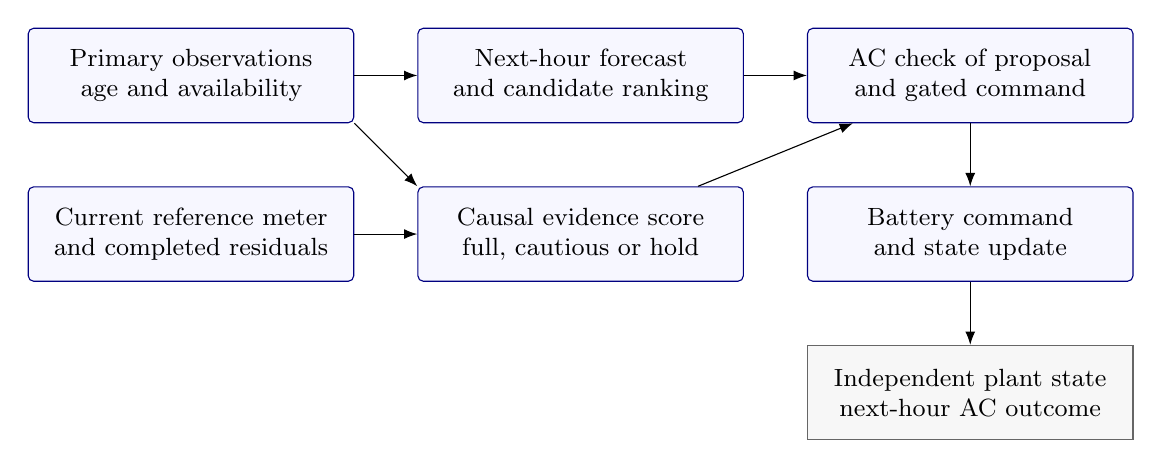
\begin{tikzpicture}[node distance=8mm and 8mm,>=Latex,
 box/.style={draw=blue!50!black,rounded corners=2pt,fill=blue!3,align=center,font=\small,minimum height=12mm,text width=39mm},
 eval/.style={draw=black!60,fill=black!3,align=center,font=\small,minimum height=12mm,text width=39mm}]
\node[box] (obs) {Primary observations\\age and availability};
\node[box,right=of obs] (pred) {Next-hour forecast\\and candidate ranking};
\node[box,right=of pred] (check) {AC check of proposal\\and gated command};
\node[box,below=of obs] (ref) {Current reference meter\\and completed residuals};
\node[box,right=of ref] (score) {Causal evidence score\\full, cautious or hold};
\node[box,right=of score] (command) {Battery command\\and state update};
\node[eval,below=of command] (plant) {Independent plant state\\next-hour AC outcome};
\draw[->] (obs)--(pred);\draw[->] (pred)--(check);
\draw[->] (obs.south east)--(score.north west);
\draw[->] (ref)--(score);\draw[->] (score)--(check);
\draw[->] (check)--(command);\draw[->] (command)--(plant);
\end{tikzpicture}
\caption{Dispatch and evaluation sequence. Current reference observations support evidence scoring. The next-hour plant state is used only for outcome evaluation.}\label{fig:architecture}
\end{figure}

\subsection{Point prediction and joint residual calibration}
The feature vector contains $z_t$, $z_{t-1}$, $z_{t-24}$, sine and cosine encodings of hour of day, and sine and cosine encodings of day of year. A multi-output random forest with 60 trees, minimum leaf size eight and feature fraction 0.75 predicts
\begin{equation}
\widehat y_{t+1|t}=f_{\theta}(z_t,z_{t-1},z_{t-24},\mathrm{calendar}_t).
\label{eq:forecast}
\end{equation}
Negative predictions are clipped to zero. The model is fitted once on the training partition; its parameters remain fixed during calibration and testing.

Let $s_j>0$ be the 90th percentile of absolute training residuals for coordinate $j\in\{\ell,g\}$, with a lower bound of $10^{-6}$. For calibration observations indexed by $i$, define
\begin{equation}
e_i=\max_{j\in\{\ell,g\}}\frac{|y_{i+1,j}-\widehat y_{i+1|i,j}|}{s_j},\quad
k=\min\{n_{\mathrm{cal}},\lceil(n_{\mathrm{cal}}+1)(1-\alpha)\rceil\},\quad \alpha=0.10.
\label{eq:calibration}
\end{equation}
If $e_{(k)}$ is the $k$th ordered calibration residual, the joint box is
\begin{equation}
\mathcal I_t=\prod_{j\in\{\ell,g\}}
[\widehat y_{t+1|t,j}-q_j,\widehat y_{t+1|t,j}+q_j],\qquad q_j=s_je_{(k)}.
\label{eq:interval}
\end{equation}
This is the standard split-calibration construction applied to a maximum residual \cite{angelopoulos}. It supplies a common joint exceedance test. Its observed coverage is reported because serial dependence and seasonal change affect interpretation \cite{oliveira}.

\subsection{Observable evidence channels}
Four channels measure different aspects of the available information. Freshness is $F_t=\exp(-a_t/2)$, with age measured in hours. Completeness is $C_t=\frac{1}{6}\sum_{s=t-5}^{t}m_s$, the fraction of primary observations available during the latest six hours. Both indicators follow from stream metadata.

Recent model performance is evaluated against reference observations whose forecast horizons have already ended. For at most 24 completed pairs in $\mathcal H_t$, define
\begin{align}
\widehat c_t&=\frac{1}{|\mathcal H_t|}\sum_{s\in\mathcal H_t}
\ind\{\max_j|r_{s,j}-\widehat y_{s|s-1,j}|/q_j\leq1\},\label{eq:recentcoverage}\\
\widehat d_t&=\frac{1}{2|\mathcal H_t|}\sum_{s\in\mathcal H_t}\sum_j
|r_{s,j}-\widehat y_{s|s-1,j}|,\label{eq:recentmae}\\
M_t&=\frac{1}{2}\min\{1,\widehat c_t/0.90\}
+\frac{1}{2}\exp[-\widehat d_t/(3d_{\mathrm{cal}})].\label{eq:maturity}
\end{align}
Here $d_{\mathrm{cal}}$ is the mean absolute calibration error averaged over both factors. At block initialisation, $\widehat c_t=0.90$ and $\widehat d_t=d_{\mathrm{cal}}$. Subsequent values use only completed reference observations. Thus a forecast made at $t$ cannot be evaluated against $r_{t+1}$ while selecting $u_t$.

Agreement between the current primary and reference measurements is
\begin{equation}
A_t=\exp\left[-\frac{|z_{t,\ell}-r_{t,\ell}|+|z_{t,g}-r_{t,g}|}{2\kappa}\right],\qquad\kappa=0.10.
\label{eq:agreement}
\end{equation}
The reference meter is assumed independent and available. Agreement tests consistency under that assumption. It does not establish source authentication or protection against a coordinated compromise of both streams.

The operating evidence score is
\begin{equation}
T_t=0.30F_t+0.25C_t+0.25M_t+0.20A_t.\label{eq:trust}
\end{equation}
All channels lie in $[0,1]$, so the score is bounded by the same interval. The weights, scales and thresholds are fixed design choices. The score has no probability interpretation. Sensitivity analysis examines these choices on held-out proposals instead of fitting them to the reported test outcomes.

\subsection{Candidate ranking and command checks}
The action set is $\mathcal U_t=\{rP^{\max}:r=-1,-0.75,\ldots,1\}$ after removing actions that violate Eq.~\eqref{eq:soc}. A local approximation of the AC solution is used for ranking. If $h(y,u)$ stacks bus voltages, branch utilisation, grid power and losses, then
\begin{equation}
\widetilde h(y,u)=h(y^0,0)+H_y(y-y^0)+H_u u,\qquad y^0=(0.6,0.4)^{\mathsf T}.\label{eq:linear}
\end{equation}
The sensitivities are calculated with separate forward perturbations of $10^{-3}$ in each factor and $10^{-3}$~MW in battery power. The approximation is fixed before testing. It uses network parameters rather than the latent next-hour plant state.

Let $v(h)$ denote the non-negative aggregate limit excess,
\begin{equation}
v(h)=\pos{0.95-\min_i V_i}+\pos{\max_i V_i-1.05}
+\pos{\max_e\rho_e-1}.\label{eq:severity}
\end{equation}
Actions are ranked by $\widetilde J_t(u)+10^5v(\widetilde h)$, where $\widetilde J_t$ uses the approximate grid power in Eq.~\eqref{eq:cost}. The first action in this order that passes the exact AC check at $\widehat y_{t+1|t}$ is the proposal $u_t^\star$. If no candidate passes, the proposal is zero and the feasibility of that hold is recorded. This finite search provides a checked recommendation; its coarse action grid and approximate ranking do not establish a global optimum.

For thresholds $\tau_L=0.65$ and $\tau_H=0.85$, the gated command is
\begin{equation}
\bar u_t=\begin{cases}
u_t^\star,&T_t\geq\tau_H,\\
0.5u_t^\star,&\tau_L\leq T_t<\tau_H,\\
0,&T_t<\tau_L.
\end{cases}\label{eq:regimes}
\end{equation}
The AC check is applied to $\bar u_t$ before it is issued. A non-zero command that fails this check is replaced by zero, and that hold is checked and logged. State of charge is updated only after command selection. A model-feasible command can still fail in the plant because $\widehat y_{t+1|t}\ne y_{t+1}$. This remaining error is the reason for independent evaluation.

\subsection{Computational implementation}
Power-flow solutions are cached by operating factors and battery power within each fixed network. State-of-charge screening remains outside the cache because action admissibility depends on the individual controller trajectory. The cache changes computational reuse rather than the information supplied to the gate. A realised-state solution can be requested only after the command has been selected. The resulting records preserve the proposal, regime, command, starting state and physical outcome at each hour. This common execution structure allows the experiments to compare gates without changing the underlying dispatch kernel.

\section{Experimental design}\label{sec:experiments}
The experiments separate temporal prediction, measurement degradation and electrical response. A common benchmark-derived operating sequence drives both networks, while each network retains its own topology, installed powers and storage size. The comparison therefore concerns the response of two electrical systems to the same quality conditions, rather than independent regional datasets.

\subsection{Networks and operating profiles}
The first network is the 33-bus distribution feeder associated with Baran and Wu \cite{baran}. Its installed load is 3.715~MW. Three unity-power-factor generators, each rated at 0.6~MW, are added at zero-based bus indices 17, 24 and 32. The battery is placed at bus index 17 and has 0.8~MW power and 3.2~MWh energy capacity. The slack voltage is 1.0~pu. The source case does not provide useful thermal ratings; a uniform line rating of 0.4~kA is therefore a study assumption. The original switch configuration is retained.

The second network is SimBench case \texttt{1-MV-rural-0-sw} \cite{meinecke}. It contains 97 buses, 99 line entries and two transformers, with 17.256~MW installed load and 25.565~MW installed generation. A 2~MW, 8~MWh battery is added at zero-based bus index 15. This bus has the highest voltage in the unmodified nameplate operating case and is selected before the profile experiments. The slack voltage is 1.025~pu. The supplied line, transformer and switching parameters are retained. Element counts include entries that are out of service or disconnected by switches.

The 2016 quarter-hourly SimBench load and renewable profiles \cite{dataset} are aggregated using each asset's installed active power as its weight. Four successive values are averaged to obtain hourly factors:
\begin{equation}
\ell_t=\frac{1}{4}\sum_{k=0}^{3}\frac{\sum_i P_i^{L}f_{i,4t+k}^{L}}{\sum_i P_i^{L}},\qquad
g_t=\frac{1}{4}\sum_{k=0}^{3}\frac{\sum_i P_i^{G}f_{i,4t+k}^{G}}{\sum_i P_i^{G}}.\label{eq:profiles}
\end{equation}
Within each network, these common factors scale the installed load and generation. This construction preserves aggregate temporal variation while imposing coherent spatial scaling. It does not reproduce the individual asset profiles at every bus. The data are benchmark profiles rather than measured operating records from an Indian or other field installation.

\subsection{Chronological partition and measurement scenarios}
Training uses January-August 2016 and calibration uses September-October 2016. Samples whose one-hour target crosses a partition boundary are removed. The final two months supply six non-overlapping 72-hour evaluation blocks starting on 1, 11 and 21 November and 1, 11 and 21 December. Each block has 24 hours of preceding primary observations for lag construction. Battery state is reset to 0.55 at the start of each block and evolves independently for each controller. Random seeds are 11, 29 and 47.

Table~\ref{tab:scenarios} specifies the six conditions. The reference stream contains independent zero-mean Gaussian noise with a standard deviation of 0.01 in each operating factor, and negative values are clipped to zero. The current reference reading is available at every decision hour. The same random seed and underlying sequence are used across controllers and networks. Fault labels are supplied only to the corruption routine and experiment log. The score routine receives the observations and their legitimate metadata.

\begin{table}[t]
\centering\small
\caption{Operating and measurement conditions applied to each evaluation block.}\label{tab:scenarios}
\begin{tabular}{p{.16\linewidth}p{.75\linewidth}}
\toprule
Condition & Definition\\\midrule
Clean & Primary observations equal the benchmark operating factors.\\
Missing & Each primary observation is unavailable with probability 0.12; both factors are carried forward from the preceding available observation.\\
Delayed & Both primary factors are delayed by two hours, with the correct age metadata.\\
Noisy & Independent Gaussian noise with standard deviation 0.08 is added to each primary factor; negative values are clipped to zero.\\
Bias & During block hours 12-17 and 48-53, the primary load factor is multiplied by 1.5 and the generation factor by 0.5.\\
Disturbance & During block hours 24-47, the actual load factor is multiplied by 1.28 and generation by 0.55; both meters observe this operating change.\\
\bottomrule
\end{tabular}
\end{table}

\subsection{Comparison controllers}
All four controllers use the same forecasting model, candidate set, tariffs, battery limits and AC command checks. The ungated controller executes the checked proposal. The metadata gate executes it only when the current observation is present and has zero age; otherwise it holds the battery. The agreement gate executes it when $A_t\geq0.65$ and holds otherwise. The trust gate uses Eq.~\eqref{eq:regimes}. Every resulting command, including a scaled action or a hold, receives the same model check and independent plant evaluation. Controller names do not enter the definition of a constraint violation.

\subsection{Operating outcomes and selective risk}
For realised state $y_{t+1}$ and command $u_t$, define $b_t=1$ if the plant power flow fails or any limit in Eq.~\eqref{eq:limits} is exceeded, and $b_t=0$ otherwise. The violation rate is
\begin{equation}
B=\frac{1}{N}\sum_{t=1}^{N}b_t.\label{eq:violations}
\end{equation}
This measure includes failures during a hold. It records whether the realised network state is feasible and does not assign every failure solely to battery control. Additional measures are mean limit excess from Eq.~\eqref{eq:severity}, total objective cost from Eq.~\eqref{eq:cost}, network energy loss and the fraction of non-zero commands. Authorisation coverage counts full or cautious regimes, including a zero recommendation that is authorised by the gate. Consequently, authorisation coverage and non-zero dispatch are reported separately.

Conditional feasible-action regret compares the realised feasible command with the least-cost feasible action in the same discrete set and at the same starting battery state:
\begin{equation}
R_t=\max\{0,J_t(u_t)-\min_{u\in\mathcal U_t:\,h(y_{t+1},u)\ \mathrm{feasible}}J_t(u)\}.\label{eq:regret}
\end{equation}
It is defined only when the issued action and at least one comparator action are plant-feasible. The comparator uses the base candidate grid, while cautious commands can take intermediate half-power values. It is a one-step retrospective comparator and does not represent an achievable controller with future knowledge. Constraint violations remain a separate outcome.

For selective-risk analysis, every test state receives one common proposal at a fixed state of charge of 0.55. This removes differences caused by earlier battery commands. For score threshold $\tau$, coverage and conditional constraint risk are
\begin{equation}
\Gamma(\tau)=\frac{1}{N}\sum_t\ind\{T_t\geq\tau\},\qquad
\mathcal R(\tau)=\frac{\sum_t b_t^{\star}\ind\{T_t\geq\tau\}}
{\sum_t\ind\{T_t\geq\tau\}},\label{eq:riskcoverage}
\end{equation}
where $b_t^{\star}$ is the realised constraint outcome of the common proposal. Risk is undefined at zero coverage. This analysis evaluates the information in a score; it does not simulate a closed-loop policy at every threshold.

\subsection{Aggregation and reproducibility}
The complete design contains 15,552 network-scenario-seed decision epochs and 62,208 controller evaluations. Each controller has 432 hours per scenario and seed on each network. Results are averaged across the six temporal blocks and three seeds. Paired differences are calculated within the same block, scenario and seed. Bootstrap uncertainty resamples whole temporal blocks, preserving all scenarios and seeds within a sampled block; individual hours are not treated as independent samples. Intervals describe variation among six sampled time blocks and have limited precision.

The implementation uses Python 3.12, pandapower 3.3.1, SimBench 1.6.3 and scikit-learn 1.7.2. The accompanying reproducibility files contain the script, aggregate hourly factors, decision records, summaries, configuration and figure data. These records support checks of the information boundary, battery updates and operating outcomes. The following section reports the resulting prediction and dispatch performance.

\section{Results}\label{sec:results}
The results first establish prediction quality on the chronological partitions and then compare complete dispatch trajectories. Selective-risk analysis uses a separate common-proposal replay, so it can reveal whether the composite score is more informative than a simpler agreement indicator. All reported constraint outcomes are obtained from realised plant states.

\subsection{Prediction quality and calibration}
Joint calibration coverage is 90.09\%, with interval half-widths of 0.03920 for load and 0.05200 for generation. On the 432 clean test hours in the selected blocks, mean absolute errors are 0.01625 and 0.01905 in the respective operating factors. Joint test coverage falls to 87.73\%. Across the complete unperturbed November-December sequence, the mean absolute error averaged over both factors is 0.01791.

The decrease from calibration to test coverage shows that a nominal residual level cannot be carried into the later seasonal partition as an unconditional guarantee. Reference-meter noise also affects the completed residuals used by the online score. For these reasons, the score represents available operating evidence, and the dispatch assessment retains the independent AC outcome as its primary feasibility measure.

\subsection{Network feasibility and control retained}
Table~\ref{tab:overall} reports the mean operating outcomes. On the 33-bus feeder, the ungated controller has 62 constraint-violating hours among 7,776 evaluated hours, compared with 30 for the trust gate. The corresponding rates are 0.797\% and 0.386\%. The agreement gate has 45 violating hours, while the metadata gate has 62. On the SimBench network, the ungated and metadata controllers each have six violating hours, the agreement gate has one, and the trust gate has none in this sample.

The trust gate authorises full or cautious dispatch during 88.99\% of decision hours. The metadata and agreement gates authorise 81.29\% and 81.07\%, respectively. These figures do not measure non-zero battery activity. Non-zero commands increase from 38.59\% to 41.01\% on the 33-bus feeder and from 18.36\% to 19.62\% on SimBench when the trust gate replaces the ungated controller. Half-power dispatch changes subsequent state of charge and can distribute storage use over more hours, even though fewer hours receive unrestricted authorisation.

All observed constraint failures concern voltage limits. The ungated 33-bus controller has 60 undervoltage and two overvoltage hours, while its trust-gated counterpart has 30 undervoltage hours. The six ungated SimBench failures are overvoltage events. No thermal-limit violation occurs in these experiments, so the observed feasibility gains relate to voltage operation.

\begin{table}[t]
\centering\small
\caption{Mean operating outcomes across equally weighted scenarios, seeds and 72-hour blocks. $B$: plant constraint violations; $\Gamma$: authorisation coverage; $U$: non-zero commands; $J$: energy-adjusted objective; $R$: conditional feasible-action regret per hour; $L$: network energy loss per block.}\label{tab:overall}
\begin{tabular}{llrrrrrr}
\toprule
Network & Controller & $B$ (\%) & $\Gamma$ (\%) & $U$ (\%) & $J$ (EUR) & $R$ (EUR) & $L$ (MWh)\\\midrule
IEEE 33 & Ungated & 0.797 & 100.00 & 38.59 & 5572.26 & 0.78 & 0.795 \\
 & Metadata gate & 0.797 & 81.29 & 31.47 & 5618.35 & 3.64 & 0.745 \\
 & Agreement gate & 0.579 & 81.07 & 33.38 & 5580.72 & 2.11 & 0.765 \\
 & Trust gate & 0.386 & 88.99 & 41.01 & 5584.42 & 2.87 & 0.699 \\
\addlinespace
SimBench MV & Ungated & 0.077 & 100.00 & 18.36 & 3463.77 & 4.27 & 3.707 \\
 & Metadata gate & 0.077 & 81.29 & 15.14 & 3640.64 & 18.44 & 3.658 \\
 & Agreement gate & 0.013 & 81.07 & 16.04 & 3523.83 & 6.99 & 3.664 \\
 & Trust gate & 0.000 & 88.99 & 19.62 & 3560.47 & 10.03 & 3.617 \\
\bottomrule\end{tabular}\end{table}
\begin{figure}[t]\centering
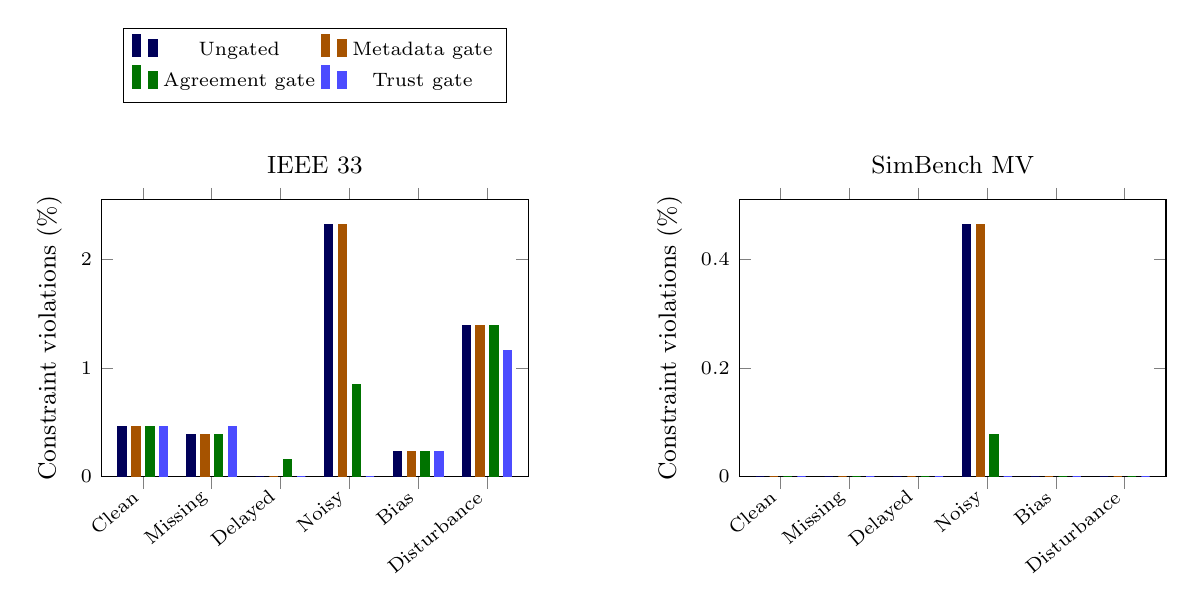
\begin{tikzpicture}
\begin{axis}[ybar,bar width=3pt,width=7.0cm,height=5.1cm,at={(0.0cm,0)},anchor=south west,ymin=0,ylabel={Constraint violations (\%)},title={IEEE 33},symbolic x coords={Clean,Missing,Delayed,Noisy,Bias,Disturbance},xtick=data,x tick label style={rotate=40,anchor=east,font=\scriptsize},tick label style={font=\scriptsize},label style={font=\small},title style={font=\small},enlarge x limits=0.12,legend style={font=\scriptsize,at={(0.5,1.35)},anchor=south,legend columns=2}]
\addplot[fill=blue!35!black,draw=blue!35!black] coordinates {(Clean,0.4629630) (Missing,0.3858025) (Delayed,0.0000000) (Noisy,2.3148148) (Bias,0.2314815) (Disturbance,1.3888889)};
\addplot[fill=orange!65!black,draw=orange!65!black] coordinates {(Clean,0.4629630) (Missing,0.3858025) (Delayed,0.0000000) (Noisy,2.3148148) (Bias,0.2314815) (Disturbance,1.3888889)};
\addplot[fill=green!45!black,draw=green!45!black] coordinates {(Clean,0.4629630) (Missing,0.3858025) (Delayed,0.1543210) (Noisy,0.8487654) (Bias,0.2314815) (Disturbance,1.3888889)};
\addplot[fill=blue!70,draw=blue!70] coordinates {(Clean,0.4629630) (Missing,0.4629630) (Delayed,0.0000000) (Noisy,0.0000000) (Bias,0.2314815) (Disturbance,1.1574074)};
\legend{Ungated,Metadata gate,Agreement gate,Trust gate}
\end{axis}
\begin{axis}[ybar,bar width=3pt,width=7.0cm,height=5.1cm,at={(8.1cm,0)},anchor=south west,ymin=0,ylabel={Constraint violations (\%)},title={SimBench MV},symbolic x coords={Clean,Missing,Delayed,Noisy,Bias,Disturbance},xtick=data,x tick label style={rotate=40,anchor=east,font=\scriptsize},tick label style={font=\scriptsize},label style={font=\small},title style={font=\small},enlarge x limits=0.12,legend style={font=\scriptsize,at={(0.5,1.35)},anchor=south,legend columns=2}]
\addplot[fill=blue!35!black,draw=blue!35!black] coordinates {(Clean,0.0000000) (Missing,0.0000000) (Delayed,0.0000000) (Noisy,0.4629630) (Bias,0.0000000) (Disturbance,0.0000000)};
\addplot[fill=orange!65!black,draw=orange!65!black] coordinates {(Clean,0.0000000) (Missing,0.0000000) (Delayed,0.0000000) (Noisy,0.4629630) (Bias,0.0000000) (Disturbance,0.0000000)};
\addplot[fill=green!45!black,draw=green!45!black] coordinates {(Clean,0.0000000) (Missing,0.0000000) (Delayed,0.0000000) (Noisy,0.0771605) (Bias,0.0000000) (Disturbance,0.0000000)};
\addplot[fill=blue!70,draw=blue!70] coordinates {(Clean,0.0000000) (Missing,0.0000000) (Delayed,0.0000000) (Noisy,0.0000000) (Bias,0.0000000) (Disturbance,0.0000000)};
\end{axis}
\end{tikzpicture}
\caption{Realised plant constraint violations by scenario. Each bar averages six 72-hour blocks and three seeds. The two panels use different vertical scales. A zero bar indicates no observed violation within the evaluated sample.}\label{fig:constraints}
\end{figure}

Figure~\ref{fig:constraints} shows that the largest observed feasibility benefit occurs under noisy measurements. On the 33-bus feeder, noise produces a 2.315\% violation rate for the ungated controller, 0.849\% for the agreement gate and zero observed violations for the trust gate. The corresponding SimBench rates are 0.463\%, 0.077\% and zero. Metadata checks alone cannot detect this condition because observations remain present and current.

The gate is not uniformly beneficial. Under missing observations on the 33-bus feeder, its violation rate is 0.463\%, compared with 0.386\% for the ungated controller. Under the physical disturbance, the rate decreases from 1.389\% to 1.157\% but remains positive. Clean-condition violations on that feeder are unchanged at 0.463\%. No feasibility improvement occurs under delay because the ungated trajectories are already feasible in the evaluated sample. These results distinguish reduced susceptibility to a defined measurement condition from a general ability to maintain network feasibility.

\subsection{Operating cost and paired uncertainty}
Mean energy-adjusted cost rises from 5,572.26 to 5,584.42~EUR per 72-hour block on the 33-bus feeder and from 3,463.77 to 3,560.47~EUR on SimBench. These increases are 12.17~EUR (0.22\%) and 96.70~EUR (2.79\%), respectively. They are averages over an equally weighted experimental mixture, not estimates based on the field frequency of faults. The agreement gate has a lower average cost than the trust gate on both networks but retains a larger physical violation rate.

The largest cost increase for the trust gate occurs under delayed measurements: 120.45~EUR per block on the 33-bus feeder and 525.28~EUR on SimBench relative to the ungated controller. No constraint violation is prevented in that condition. In contrast, under noise, its cost is lower by 44.88 and 9.17~EUR, respectively. Mean conditional feasible-action regret increases with the trust gate, indicating a cost of restricting or scaling an otherwise useful checked proposal. Regret excludes infeasible issued actions and must be read together with the violation rate.

\begin{table}[t]
\centering\small
\caption{Paired trust-gate differences relative to the ungated controller. Brackets show percentile 95\% bootstrap intervals from 10,000 resamples of six whole temporal blocks. Rates are in percentage points (pp), and costs are in EUR per 72-hour block.}\label{tab:paired}
\begin{tabular}{llrr}
\toprule
Network & Outcome & Mean difference & Bootstrap interval\\\midrule
IEEE 33 & Constraint violations (pp) & -0.412 & [-0.630, -0.193] \\
 & Energy-adjusted cost (EUR) & 12.166 & [-2.171, 25.503] \\
 & Non-zero commands (pp) & 2.418 & [0.849, 3.871] \\
\addlinespace
SimBench MV & Constraint violations (pp) & -0.077 & [-0.206, 0.000] \\
 & Energy-adjusted cost (EUR) & 96.697 & [50.474, 137.512] \\
 & Non-zero commands (pp) & 1.260 & [-0.373, 2.932] \\
\bottomrule\end{tabular}\end{table}

Table~\ref{tab:paired} gives paired block-bootstrap intervals. The 33-bus violation-rate difference is -0.412 percentage points, with an interval from -0.630 to -0.193. The SimBench difference is -0.077 percentage points, with an interval reaching zero. Its small event count therefore supports only a limited conclusion. The cost interval on the 33-bus feeder includes zero, whereas the SimBench interval remains positive. These intervals preserve dependence within temporal blocks but are based on six blocks and should not be interpreted as broad population guarantees.

Mean network energy loss decreases from 0.795 to 0.699~MWh per block on the 33-bus feeder and from 3.707 to 3.617~MWh on SimBench. Lower network loss does not imply a lower overall objective because the latter also includes tariff timing, throughput and stored-energy value. Together, the operating measures show how the gate changes the use of storage rather than reducing all losses by a common amount.

\subsection{Selective risk and score sensitivity}
Figure~\ref{fig:risk} compares scores on common proposals. At matched 90\% coverage under degraded conditions, selective violation risk on the 33-bus feeder is 2.023\% for the trust score and 1.886\% for the agreement score. At 75\% coverage, the rates are 1.790\% and 1.646\%; at 50\%, they are 1.481\% and 1.265\%. On SimBench, the corresponding pairs are 0.120\% and 0.034\%, 0.062\% and 0.021\%, and zero for both scores. Thus the combined score does not provide better selective ranking than agreement alone at these operating points.

\begin{figure}[t]\centering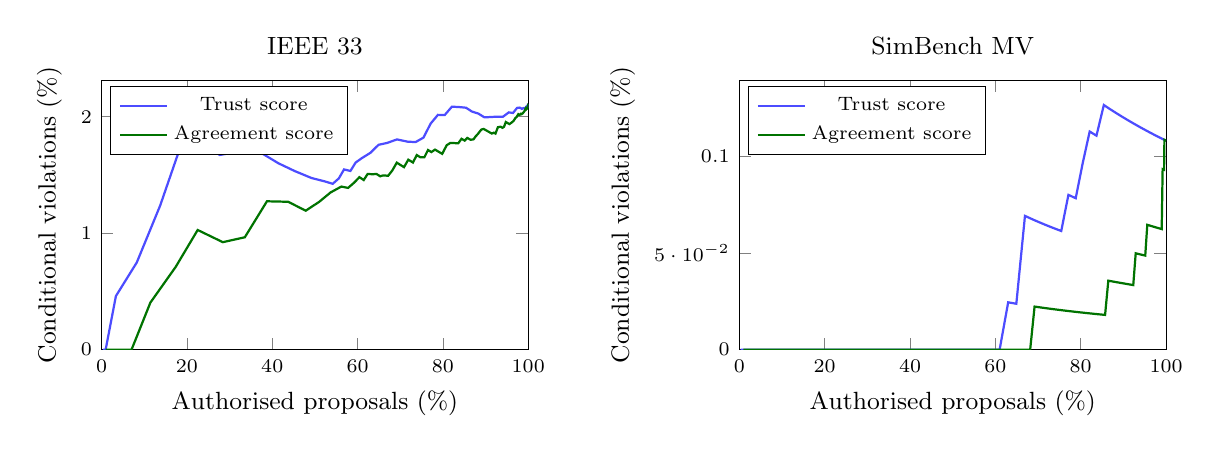
\begin{tikzpicture}
\begin{axis}[width=7.0cm,height=5cm,at={(0.0cm,0)},anchor=south west,xmin=0,xmax=100,ymin=0,xlabel={Authorised proposals (\%)},ylabel={Conditional violations (\%)},title={IEEE 33},tick label style={font=\scriptsize},label style={font=\small},title style={font=\small},legend style={font=\scriptsize,at={(0.02,0.98)},anchor=north west}]
\addplot[thick,color=blue!70] coordinates {(100.00000,2.0987654) (100.00000,2.0987654) (100.00000,2.0987654) (100.00000,2.0987654) (100.00000,2.0987654) (100.00000,2.0987654) (100.00000,2.0987654) (100.00000,2.0987654) (100.00000,2.0987654) (100.00000,2.0987654) (100.00000,2.0987654) (100.00000,2.0987654) (100.00000,2.0987654) (100.00000,2.0987654) (100.00000,2.0987654) (100.00000,2.0987654) (100.00000,2.0987654) (100.00000,2.0987654) (100.00000,2.0987654) (100.00000,2.0987654) (100.00000,2.0987654) (100.00000,2.0987654) (100.00000,2.0987654) (100.00000,2.0987654) (100.00000,2.0987654) (100.00000,2.0987654) (100.00000,2.0987654) (100.00000,2.0987654) (100.00000,2.0987654) (100.00000,2.0987654) (100.00000,2.0987654) (100.00000,2.0987654) (100.00000,2.0987654) (100.00000,2.0987654) (100.00000,2.0987654) (100.00000,2.0987654) (100.00000,2.0987654) (100.00000,2.0987654) (100.00000,2.0987654) (100.00000,2.0987654) (100.00000,2.0987654) (100.00000,2.0987654) (99.98457,2.0990894) (99.98457,2.0990894) (99.98457,2.0990894) (99.98457,2.0990894) (99.98457,2.0990894) (99.96914,2.0994134) (99.92284,2.1003861) (99.90741,2.1007105) (99.81481,2.0871985) (99.64506,2.0907542) (99.41358,2.0800993) (99.19753,2.0690728) (98.91975,2.0748830) (98.50309,2.0679931) (97.99383,2.0787402) (97.37654,2.0760697) (96.41975,2.0326504) (95.43210,2.0375162) (94.08951,2.0009841) (92.56173,2.0006669) (91.15741,1.9976299) (89.72222,1.9951840) (88.28704,2.0276175) (86.79012,2.0448080) (85.41667,2.0776874) (83.68827,2.0837175) (82.09877,2.0864662) (80.41667,2.0149683) (78.82716,2.0164448) (77.11420,1.9411647) (75.43210,1.8207856) (73.58025,1.7827181) (71.69753,1.7864830) (69.22840,1.8056175) (66.92901,1.7754208) (64.90741,1.7593913) (62.99383,1.6903479) (60.98765,1.6447368) (59.53704,1.6070503) (58.31790,1.5347976) (56.82099,1.5480717) (55.60185,1.4709964) (54.16667,1.4245014) (52.33025,1.4450015) (49.19753,1.4742785) (45.27778,1.5337423) (41.46605,1.6002977) (37.48457,1.6879374) (32.60802,1.7037388) (27.68519,1.6722408) (23.42593,1.7786561) (18.53395,1.7485429) (13.71914,1.2373453) (8.24074,0.7490637) (3.34877,0.4608295) (0.94136,0.0000000) (0.29321,0.0000000)};
\addplot[thick,color=green!45!black] coordinates {(100.00000,2.0987654) (100.00000,2.0987654) (100.00000,2.0987654) (100.00000,2.0987654) (100.00000,2.0987654) (100.00000,2.0987654) (100.00000,2.0987654) (100.00000,2.0987654) (100.00000,2.0987654) (100.00000,2.0987654) (100.00000,2.0987654) (100.00000,2.0987654) (100.00000,2.0987654) (99.98457,2.0990894) (99.98457,2.0990894) (99.98457,2.0990894) (99.95370,2.0842983) (99.87654,2.0704574) (99.79938,2.0720581) (99.73765,2.0733406) (99.61420,2.0759101) (99.53704,2.0775194) (99.44444,2.0639354) (99.32099,2.0665009) (99.19753,2.0535159) (98.98148,2.0424072) (98.75000,2.0315674) (98.45679,2.0219436) (98.27160,2.0257538) (97.97840,2.0160655) (97.66975,2.0224364) (97.28395,1.9987310) (96.97531,1.9891789) (96.57407,1.9654842) (96.28086,1.9554416) (95.94136,1.9462763) (95.60185,1.9370460) (95.12346,1.9467878) (94.73765,1.9547158) (94.32099,1.9142670) (93.95062,1.9053876) (93.50309,1.9145073) (92.88580,1.9106164) (92.31481,1.8555667) (91.92901,1.8633540) (91.46605,1.8559136) (91.06481,1.8640908) (90.47840,1.8761726) (89.92284,1.8877639) (89.55247,1.8955713) (88.99691,1.8900642) (88.22531,1.8541193) (87.65432,1.8309859) (87.16049,1.8059490) (86.46605,1.8026057) (85.70988,1.8185092) (85.09259,1.7954298) (84.35185,1.8111965) (83.59568,1.7721986) (82.63889,1.7740430) (81.71296,1.7752597) (80.87963,1.7553902) (79.83025,1.6818094) (78.90432,1.7015451) (78.14815,1.7180095) (77.28395,1.6972843) (76.49691,1.7147468) (75.64815,1.6523868) (74.75309,1.6515277) (73.87346,1.6711928) (72.96296,1.6074450) (71.88272,1.6316015) (70.87963,1.5676029) (70.01543,1.5869517) (69.18210,1.6060674) (68.14815,1.5398551) (67.16049,1.4935662) (65.98765,1.4967259) (65.29321,1.4890097) (64.41358,1.5093436) (63.51852,1.5063168) (62.36111,1.5095273) (61.43519,1.4569204) (60.41667,1.4814815) (59.18210,1.4341591) (57.76235,1.3892600) (56.18827,1.4007141) (53.68827,1.3509629) (51.01852,1.2704174) (47.83951,1.1935484) (43.73457,1.2702893) (38.75000,1.2743927) (33.56481,0.9655172) (28.41049,0.9234112) (22.51543,1.0281014) (17.36111,0.7111111) (11.43519,0.4048583) (7.00617,0.0000000) (3.04012,0.0000000) (0.94136,0.0000000)};
\legend{Trust score,Agreement score}\end{axis}
\begin{axis}[width=7.0cm,height=5cm,at={(8.1cm,0)},anchor=south west,xmin=0,xmax=100,ymin=0,xlabel={Authorised proposals (\%)},ylabel={Conditional violations (\%)},title={SimBench MV},tick label style={font=\scriptsize},label style={font=\small},title style={font=\small},legend style={font=\scriptsize,at={(0.02,0.98)},anchor=north west}]
\addplot[thick,color=blue!70] coordinates {(100.00000,0.1080247) (100.00000,0.1080247) (100.00000,0.1080247) (100.00000,0.1080247) (100.00000,0.1080247) (100.00000,0.1080247) (100.00000,0.1080247) (100.00000,0.1080247) (100.00000,0.1080247) (100.00000,0.1080247) (100.00000,0.1080247) (100.00000,0.1080247) (100.00000,0.1080247) (100.00000,0.1080247) (100.00000,0.1080247) (100.00000,0.1080247) (100.00000,0.1080247) (100.00000,0.1080247) (100.00000,0.1080247) (100.00000,0.1080247) (100.00000,0.1080247) (100.00000,0.1080247) (100.00000,0.1080247) (100.00000,0.1080247) (100.00000,0.1080247) (100.00000,0.1080247) (100.00000,0.1080247) (100.00000,0.1080247) (100.00000,0.1080247) (100.00000,0.1080247) (100.00000,0.1080247) (100.00000,0.1080247) (100.00000,0.1080247) (100.00000,0.1080247) (100.00000,0.1080247) (100.00000,0.1080247) (100.00000,0.1080247) (100.00000,0.1080247) (100.00000,0.1080247) (100.00000,0.1080247) (100.00000,0.1080247) (100.00000,0.1080247) (99.98457,0.1080414) (99.98457,0.1080414) (99.98457,0.1080414) (99.98457,0.1080414) (99.98457,0.1080414) (99.96914,0.1080580) (99.92284,0.1081081) (99.90741,0.1081248) (99.81481,0.1082251) (99.64506,0.1084095) (99.41358,0.1086619) (99.19753,0.1088986) (98.91975,0.1092044) (98.50309,0.1096663) (97.99383,0.1102362) (97.37654,0.1109350) (96.41975,0.1120359) (95.43210,0.1131953) (94.08951,0.1148106) (92.56173,0.1167056) (91.15741,0.1185035) (89.72222,0.1203990) (88.28704,0.1223562) (86.79012,0.1244666) (85.41667,0.1264679) (83.68827,0.1106399) (82.09877,0.1127820) (80.41667,0.0959509) (78.82716,0.0783085) (77.11420,0.0800480) (75.43210,0.0613748) (73.58025,0.0629195) (71.69753,0.0645717) (69.22840,0.0668747) (66.92901,0.0691722) (64.90741,0.0237756) (62.99383,0.0244978) (60.98765,0.0000000) (59.53704,0.0000000) (58.31790,0.0000000) (56.82099,0.0000000) (55.60185,0.0000000) (54.16667,0.0000000) (52.33025,0.0000000) (49.19753,0.0000000) (45.27778,0.0000000) (41.46605,0.0000000) (37.48457,0.0000000) (32.60802,0.0000000) (27.68519,0.0000000) (23.42593,0.0000000) (18.53395,0.0000000) (13.71914,0.0000000) (8.24074,0.0000000) (3.34877,0.0000000) (0.94136,0.0000000) (0.29321,0.0000000)};
\addplot[thick,color=green!45!black] coordinates {(100.00000,0.1080247) (100.00000,0.1080247) (100.00000,0.1080247) (100.00000,0.1080247) (100.00000,0.1080247) (100.00000,0.1080247) (100.00000,0.1080247) (100.00000,0.1080247) (100.00000,0.1080247) (100.00000,0.1080247) (100.00000,0.1080247) (100.00000,0.1080247) (100.00000,0.1080247) (99.98457,0.1080414) (99.98457,0.1080414) (99.98457,0.1080414) (99.95370,0.1080747) (99.87654,0.1081582) (99.79938,0.1082418) (99.73765,0.1083088) (99.61420,0.1084431) (99.53704,0.0930233) (99.44444,0.0931099) (99.32099,0.0932256) (99.19753,0.0933416) (98.98148,0.0623636) (98.75000,0.0625098) (98.45679,0.0626959) (98.27160,0.0628141) (97.97840,0.0630020) (97.66975,0.0632011) (97.28395,0.0634518) (96.97531,0.0636537) (96.57407,0.0639182) (96.28086,0.0641128) (95.94136,0.0643397) (95.60185,0.0645682) (95.12346,0.0486697) (94.73765,0.0488679) (94.32099,0.0490838) (93.95062,0.0492773) (93.50309,0.0495131) (92.88580,0.0498422) (92.31481,0.0334336) (91.92901,0.0335739) (91.46605,0.0337439) (91.06481,0.0338926) (90.47840,0.0341122) (89.92284,0.0343230) (89.55247,0.0344649) (88.99691,0.0346801) (88.22531,0.0349834) (87.65432,0.0352113) (87.16049,0.0354108) (86.46605,0.0356952) (85.70988,0.0180050) (85.09259,0.0181357) (84.35185,0.0182949) (83.59568,0.0184604) (82.63889,0.0186741) (81.71296,0.0188857) (80.87963,0.0190803) (79.83025,0.0193311) (78.90432,0.0195580) (78.14815,0.0197472) (77.28395,0.0199681) (76.49691,0.0201735) (75.64815,0.0203998) (74.75309,0.0206441) (73.87346,0.0208899) (72.96296,0.0211506) (71.88272,0.0214684) (70.87963,0.0217723) (70.01543,0.0220410) (69.18210,0.0223065) (68.14815,0.0000000) (67.16049,0.0000000) (65.98765,0.0000000) (65.29321,0.0000000) (64.41358,0.0000000) (63.51852,0.0000000) (62.36111,0.0000000) (61.43519,0.0000000) (60.41667,0.0000000) (59.18210,0.0000000) (57.76235,0.0000000) (56.18827,0.0000000) (53.68827,0.0000000) (51.01852,0.0000000) (47.83951,0.0000000) (43.73457,0.0000000) (38.75000,0.0000000) (33.56481,0.0000000) (28.41049,0.0000000) (22.51543,0.0000000) (17.36111,0.0000000) (11.43519,0.0000000) (7.00617,0.0000000) (3.04012,0.0000000) (0.94136,0.0000000)};
\legend{Trust score,Agreement score}\end{axis}
\end{tikzpicture}
\caption{Selective constraint risk on common proposals at a fixed state of charge of 0.55, excluding the clean scenario. Thresholds vary from 0 to 0.99. These curves assess score selection rather than complete battery trajectories. Panels use different vertical scales.}\label{fig:risk}
\end{figure}
\begin{table}[t]\centering\small
\caption{Threshold and weight sensitivity on common proposals under degraded conditions. Coverage is identical for the two networks because their scores use the same factors. Risk is conditional on selection and is reported in percent. No cautious scaling or state evolution is applied in this replay.}\label{tab:sensitivity}
\begin{tabular}{lrrrr}
\toprule
Score design & Threshold & Coverage (\%) & IEEE 33 risk (\%) & SimBench risk (\%)\\\midrule
Default & 0.65 & 86.79 & 2.045 & 0.124 \\
Default & 0.75 & 69.23 & 1.806 & 0.067 \\
Default & 0.85 & 52.33 & 1.445 & 0.000 \\
Default & 0.95 & 8.24 & 0.749 & 0.000 \\
Equal weights & 0.85 & 50.73 & 1.430 & 0.000 \\
Freshness emphasis & 0.85 & 56.50 & 1.502 & 0.000 \\
No freshness & 0.85 & 36.59 & 1.603 & 0.000 \\
\bottomrule\end{tabular}\end{table}

Table~\ref{tab:sensitivity} reports the selection effect of threshold and weight changes. At threshold 0.85, default weights retain 52.33\% of degraded-condition proposals and give a 1.445\% conditional violation risk on the 33-bus feeder. Equal weights retain 50.73\% with 1.430\% risk. Freshness-emphasised weights retain 56.50\% with 1.502\% risk. Removing freshness and normalising the remaining weights retains 36.59\% with 1.603\% risk. The removed-channel design changes the scale as well as the information content, so this last comparison is a sensitivity result rather than an isolated causal effect of freshness. The default setting is not selected as an optimum from these test outcomes.

The common-proposal findings qualify the trajectory results. The closed-loop feasibility benefit of the trust gate cannot be attributed solely to superior fault ranking. Cautious scaling and the resulting battery-state trajectory are also involved. This distinction forms the basis for interpreting the method's operational role and limitations.


\section{Discussion}\label{sec:discussion}
The proposed gate changes the degree of dispatch rather than replacing the physical network model. Its strongest observed benefit is associated with noisy measurements, where scaling can limit an unsuitable action while preserving storage for later hours. The evidence also identifies conditions in which gating has little benefit or adds avoidable cost. These outcomes determine where a supervisory gate may be useful and where a simpler indicator deserves preference.

\subsection{Meaning of trust in the dispatch layer}
The score combines metadata and measured residual evidence into an operating rule. It is neither a calibrated probability of feasibility nor a certificate of measurement integrity. The agreement channel provides particularly useful information in the defined corruption tests because the reference stream remains independent and available. Its lower selective risk at matched coverage shows that the additional channels do not automatically improve decision ranking. Their practical value must be established for the quality conditions expected at a particular installation.

The benefit of cautious control is also state dependent. Scaling a discharge reduces immediate voltage support, while scaling a charge can reduce the associated voltage drop. The AC recheck therefore remains necessary after applying the gate. A hold preserves battery energy but can leave an already stressed network outside its voltage limits. The positive violation rate during the physical disturbance demonstrates that this distinction affects the reported outcomes.

\subsection{Implications for sustainable network operation}
Measurement-quality control can support storage operation by avoiding some commands derived from unreliable state estimates. In the evaluated noise condition, lower constraint violations occur together with lower energy-adjusted cost. Across the full scenario mixture, however, the trust gate carries an economic penalty. A network operator would therefore need to select a dispatch regime using the consequences of a missed action, the cost of a hold and the expected measurement conditions.

The reduction in network energy loss is a secondary operating result. Renewable curtailment, carbon emissions, battery ageing beyond the fixed throughput charge and long-term economic return are not evaluated. The results therefore concern battery dispatch and electrical feasibility under the specified benchmark conditions. Extending the operating objective to those additional quantities would require their explicit models and data.

\subsection{Limits of the evidence}
The plant and controller share topology and electrical parameters. Their difference arises from operating-factor estimates, so the study does not measure robustness to parameter drift, incorrect switching states or unbalanced phase conditions. Common aggregate factors also suppress spatial diversity among loads and generators. Testing the original asset-specific profiles would reveal whether the gate retains its behaviour when local power injections vary independently.

The reference stream is a strong deployment assumption. A coordinated bias in both meters can preserve agreement while changing the estimated state, and a missing reference would remove both agreement and completed-residual evidence. The experiments cover neither condition. A deployed controller would need a defined treatment of reference availability, source validation and local protective functions.

The dispatch kernel uses one battery, nine candidate levels and a one-hour objective. It does not impose a multi-hour terminal state, model converter transients or coordinate reactive power. Multi-period optimisation and hardware-in-the-loop evaluation would test interactions that are absent here. In addition, all test blocks lie in the final two months of one benchmark year. Six temporal clusters and three measurement seeds provide reproducible comparisons but limited evidence for seasonal and geographic transfer. These boundaries lead to a conclusion centred on demonstrated operating trade-offs rather than universal performance.


\section{Conclusion}\label{sec:conclusion}
A causal trust gate has been developed for battery dispatch using measurement freshness, completeness, completed forecast residuals and independent meter agreement. Candidate and scaled commands are checked against the estimated AC network before execution, and realised plant feasibility is evaluated separately. Experiments on a 33-bus feeder and a 97-bus SimBench network show fewer constraint violations under the specified noisy-measurement condition. Across all tested conditions, the gate reduces violation rates while increasing mean energy-adjusted cost and changing the battery-state trajectory.

The results also establish clear limits. Holding storage does not ensure a feasible network state, and the composite score does not outperform agreement alone in the matched-coverage selective-risk comparison. The method is therefore supported as a measurable supervisory dispatch mechanism with a cost-feasibility trade-off. Asset-specific spatial profiles, unreliable reference streams and multi-period control provide the next validation steps for practical deployment.

\section*{Data availability}
The network and source profile data are available through SimBench and pandapower \cite{meinecke,thurner}. Aggregate hourly factors, experiment code, decision records and figure data accompany this article as reproducibility material. The package records the model settings, random seeds and chronological partitions used to obtain the reported results.

\appendix
\section{Implementation checks}\label{sec:checks}
The evaluation contract is checked at the level of individual decisions. Battery state is recalculated from each command using Eq.~\eqref{eq:soc}; states outside the prescribed interval are counted as implementation failures. Scores are recalculated from the four saved channels and the fixed weights. Authorisation labels are compared with Eq.~\eqref{eq:regimes}, and physical violation labels are derived from the saved plant voltages and branch limits, without using controller names. Cached power-flow states are also compared with fresh network solutions for a sample of operating points. These checks assess implementation consistency and are distinct from evidence about the quality of a control policy.

\begin{thebibliography}{99}
\small\raggedright
\bibitem{ardebili} A. Aghazadeh Ardebili, M. Zappatore, A.I.H.A. Ramadan, A. Longo, A. Ficarella, Digital Twins of smart energy systems: a systematic literature review on enablers, design, management and computational challenges, Energy Informatics 7 (2024) 94. \href{https://doi.org/10.1186/s42162-024-00385-5}{doi:10.1186/s42162-024-00385-5}.
\bibitem{hueros} P.J. Hueros-Barrios, J. Espolio-Maestro, S. Rodr\'iguez-Carrasco, C. Santos-P\'erez, F.J. Rodr\'iguez-S\'anchez, P. Mart\'in S\'anchez, M. Tradacete-\'Agreda, F. Blaabjerg, Real-time digital twin prototype for cyber-physical analysis of anomalies in PV-PEM-BESS systems for green hydrogen production, Sustainable Energy, Grids and Networks 45 (2026) 102152. \href{https://doi.org/10.1016/j.segan.2026.102152}{doi:10.1016/j.segan.2026.102152}.
\bibitem{zhang} X. Zhang, D.K.J. Lin, L. Wang, Digital twin optimization: A sequential approach, Computers \& Industrial Engineering 208 (2025) 111235. \href{https://doi.org/10.1016/j.cie.2025.111235}{doi:10.1016/j.cie.2025.111235}.
\bibitem{panda} S.P. Panda, B. Genest, A. Easwaran, R. Rigo-Mariani, P. Lin, Methods for mitigating uncertainty in real-time operations of a connected microgrid, Sustainable Energy, Grids and Networks 38 (2024) 101334. \href{https://doi.org/10.1016/j.segan.2024.101334}{doi:10.1016/j.segan.2024.101334}.
\bibitem{rahman} D.M. Rahman, S. Ganguly, Voltage regulation and energy loss minimization for distribution networks with high photovoltaic penetration and EV charging stations using dual-stage model predictive control, Sustainable Energy, Grids and Networks 40 (2024) 101529. \href{https://doi.org/10.1016/j.segan.2024.101529}{doi:10.1016/j.segan.2024.101529}.
\bibitem{li} L. Li, Y. Ju, Z. Wang, Quantifying the impact of building load forecasts on optimizing energy storage systems, Energy and Buildings 307 (2024) 113913. \href{https://doi.org/10.1016/j.enbuild.2024.113913}{doi:10.1016/j.enbuild.2024.113913}.
\bibitem{breiman} L. Breiman, Random forests, Machine Learning 45 (2001) 5-32. \href{https://doi.org/10.1023/A:1010933404324}{doi:10.1023/A:1010933404324}.
\bibitem{angelopoulos} A.N. Angelopoulos, S. Bates, Conformal prediction: A gentle introduction, Foundations and Trends in Machine Learning 16 (2023) 494-591. \href{https://doi.org/10.1561/2200000101}{doi:10.1561/2200000101}.
\bibitem{oliveira} R.I. Oliveira, P. Orenstein, T. Ramos, J.V. Romano, Split conformal prediction and non-exchangeable data, Journal of Machine Learning Research 25 (225) (2024) 1-38. \url{https://jmlr.org/papers/v25/23-1553.html}.
\bibitem{gibbs} I. Gibbs, E.J. Cand\`es, Conformal inference for online prediction with arbitrary distribution shifts, Journal of Machine Learning Research 25 (162) (2024) 1-36. \url{https://jmlr.org/papers/v25/22-1218.html}.
\bibitem{liu} Y. Liu, P. Ning, M.K. Reiter, False data injection attacks against state estimation in electric power grids, ACM Transactions on Information and System Security 14 (1) (2011) 1-33. \href{https://doi.org/10.1145/1952982.1952995}{doi:10.1145/1952982.1952995}.
\bibitem{pasqualetti} F. Pasqualetti, F. D\"orfler, F. Bullo, Attack detection and identification in cyber-physical systems, IEEE Transactions on Automatic Control 58 (2013) 2715-2729. \href{https://doi.org/10.1109/TAC.2013.2266831}{doi:10.1109/TAC.2013.2266831}.
\bibitem{dongliu} D. Liu, S. Timmerman, Y. Xiang, E. Hosseini, P. Palensky, P.P. Vergara, A data-driven approach for topology correction in low voltage distribution networks with photovoltaics, Sustainable Energy, Grids and Networks 46 (2026) 102321. \href{https://doi.org/10.1016/j.segan.2026.102321}{doi:10.1016/j.segan.2026.102321}.
\bibitem{baran} M.E. Baran, F.F. Wu, Network reconfiguration in distribution systems for loss reduction and load balancing, IEEE Transactions on Power Delivery 4 (1989) 1401-1407. \href{https://doi.org/10.1109/61.25627}{doi:10.1109/61.25627}.
\bibitem{meinecke} S. Meinecke, D. Sarajli\'c, S.R. Drauz, A. Klettke, L.-P. Lauven, C. Rehtanz, A. Moser, M. Braun, SimBench: A benchmark dataset of electric power systems to compare innovative solutions based on power flow analysis, Energies 13 (2020) 3290. \href{https://doi.org/10.3390/en13123290}{doi:10.3390/en13123290}.
\bibitem{thurner} L. Thurner, A. Scheidler, F. Sch\"afer, J.-H. Menke, J. Dollichon, F. Meier, S. Meinecke, M. Braun, pandapower: An open-source Python tool for convenient modeling, analysis, and optimization of electric power systems, IEEE Transactions on Power Systems 33 (2018) 6510-6521. \href{https://doi.org/10.1109/TPWRS.2018.2829021}{doi:10.1109/TPWRS.2018.2829021}.
\bibitem{dataset} [dataset] SimBench, Power-system benchmark data and 2016 operating profiles, case \texttt{1-MV-rural--0-sw}, distributed with SimBench 1.6.3. \url{https://simbench.de/en/download/datasets/} (accessed 6 October 2026).
\end{thebibliography}
\end{document}
